 \providecommand{\main}{../../..}
\documentclass[\main/main.tex]{subfiles}
\begin{document}
\subsection{Esercizio 2}
Dato il seguente problema di PL, calcolare il duale, verificare mediante \textbf{scarti complementari} se $x=(0,0,3,\frac{1}{2})$ è ottima e riportare il vettore della soluzione duale corrispondente.

\begin{figure}
  \begin{align*}
    \min \quad 2x_1 + 5x_2 + x_3 + x4 \\
    x_1 - x_2 + x_3  & = 3            \\
    x_1 + x_3 + 2x_4 & = 4            \\
    x_1,x_2,x_3,x_4  & \geq 0
  \end{align*}
  \caption{Esercizio 2}
\end{figure}

\subsection{Soluzione esercizio 2}
\subsubsection*{Problema duale}
\begin{enumerate}
  \item P è un problema di minimo, quindi D sarà di massimo.
  \item La z di P è in funzione di 4 variabili, quindi D avrà 4 vincoli.
  \item P ha 2 vincoli di uguaglianza, per cui D avrà due variabili libere $\omega_1, \omega_2 \in \mathbb{R}$ in segno o 4 accoppiate positive $\omega_1 = y_1 - y_2, \omega_2 = y_3 - y_4, \text{con} y_1, y_2, y_3, y_4 \geq 0$.
\end{enumerate}

\begin{figure}
  \begin{subfigure}{0.49\textwidth}
    \begin{align*}
      \max \quad 3\omega_1 + 4\omega_2     \\
      \omega_1 + \omega_2 & \leq 2         \\
      -\omega_1           & \leq 5         \\
      \omega_1 + \omega_2 & \leq 1         \\
      2\omega_2           & \leq 1         \\
      \omega_1, \omega_2  & \in \mathbb{R}
    \end{align*}
    \caption{Duale con variabili libere}
  \end{subfigure}
  \begin{subfigure}{0.49\textwidth}
    \begin{align*}
      \max \quad 3(y_1 - y_2) + 4(y_3 - y_4) \\
      (y_1 - y_2) + (y_3 - y_4) & \leq 2     \\
      -(y_1 - y_2)              & \leq 5     \\
      (y_1 - y_2) + (y_3 - y_4) & \leq 1     \\
      2(y_3 - y_4)              & \leq 1     \\
      y_1, y_2, y_3, y_4        & \geq 0
    \end{align*}
    \caption{Duale con variabili positive}
  \end{subfigure}
  \caption{Problema duale}
\end{figure}

\subsubsection*{Scarti complementari}
\begin{figure}
  \begin{subfigure}{0.31\textwidth}
    \begin{align*}
      \omega_1(x_1 - x_2 + x_3 - 3) = 0 \\
      \omega_2(x_1 + x_3 + 2x_4 -4) = 0 \\
      x_1(\omega_1 + \omega_2 -2) = 0   \\
      x_2(-\omega_1-5)=0                \\
      x_3(\omega_1 + \omega_2-1)=0      \\
      x_4(2\omega_2-1)=0                \\
    \end{align*}
    \caption{Imposto sistema}
  \end{subfigure}
  \begin{subfigure}{0.31\textwidth}
    \begin{align*}
      \omega_1(0 - 0 + 3 - 3) = 0           \\
      \omega_2(0 + 3 + 2\frac{1}{2} -4) = 0 \\
      0(\omega_1 + \omega_2 -2) = 0         \\
      0(-\omega_1-5)=0                      \\
      3(\omega_1 + \omega_2-1)=0            \\
      \frac{1}{2}(2\omega_2-1)=0            \\
    \end{align*}
    \caption{Sostituisco i valori della soluzione}
  \end{subfigure}
  \begin{subfigure}{0.31\textwidth}
    \begin{align*}
      \omega_1=\frac{1}{2} \\
      \omega_2=\frac{1}{2} \\
    \end{align*}
    \caption{Semplifico}
  \end{subfigure}
  \caption{Scarti complementari}
\end{figure}

Il sistema ha soluzione, per cui la soluzione proposta $x=(0,0,3,\frac{1}{2})$ è ottima.

\subsubsection*{Vettore della soluzione duale in corrisponsenza dell'ottimo}
Indico le variabili di \textit{slack} dei 4 vincoli come $s_1, s_2, s_3$ e $s_4$:

\begin{align*}
  \omega_1 & = \frac{1}{2}  \\
  \omega_2 & = \frac{1}{2}  \\
  s_1      & = 1            \\
  s_2      & = -\frac{9}{2} \\
  s_3      & = 0            \\
  s_4      & = 0            \\
\end{align*}

\subsubsection*{Verifico le soluzioni ottenute}
Non potendo plottare il grafico di $P$ essendo in $4$ variabili vado a disegnare il duale.

\begin{figure}
  \begin{subfigure}{0.45\textwidth}
    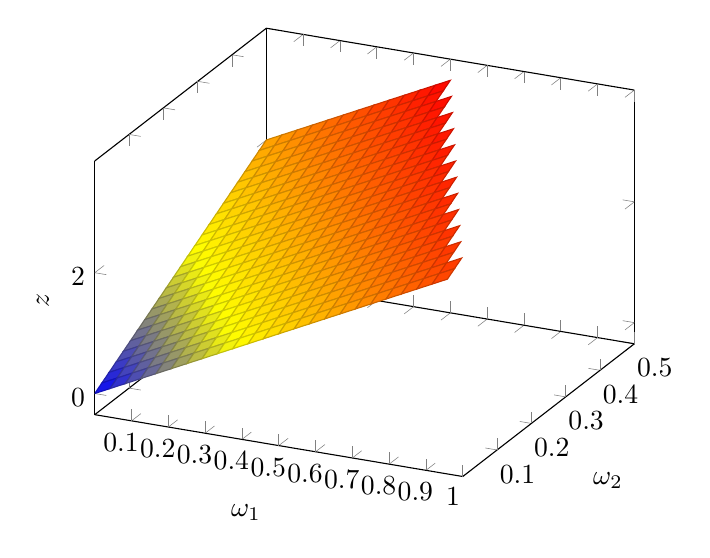
\begin{tikzpicture}
      \begin{axis}[
          xlabel=$\omega_1$,
          ylabel=$\omega_2$,
          zlabel=$z$,
          domain=0:1,
          y domain= 0:0.5,
          ytick={0.1,0.2,...,0.5},
          xtick={0.1,0.2,...,1}
        ]
        \addplot3[surf, unbounded coords=jump]
        {
          x + y <= 2 &&
          -x <= 5 &&
          x + y <= 1 &&
          2*y <= 1 ?
          3*x + 4*y:NaN
        };
      \end{axis}
    \end{tikzpicture}
    \caption{La funzione $z$ del problema $D$}
  \end{subfigure}
\end{figure}

Nel grafico duale appare $(\frac{1}{2}, \frac{1}{2})$ come soluzione ottima.

\end{document}